\documentclass[a4paper]{article}
\usepackage{geometry}
 \geometry{
 a4paper,
 total={170mm,257mm},
 left=35mm, right=30mm,
 top=20mm,bottom=13mm
 }
\usepackage{bm}					% Bold Greek letters in math mode.
\usepackage{bbm}
\usepackage{graphicx}
\usepackage{amsmath,amsfonts,amssymb,mathtools}	
\usepackage{cancel}
\usepackage{latexsym} 			
\usepackage{subcaption}
\usepackage{float}
\usepackage{tikz}
\usepackage{ifthen}
\usepackage{neuralnetwork}


%\usepackage[rightcaption]{sidecap}
%\newcommand{\xmark}{\ding{55}}
%\newenvironment{tightcenter}{%
%  \setlength\topsep{0pt}
%  \setlength\parskip{0pt}
%  \begin{center}
%}{%
% \end{center}
%}
%% ----------------------------------------------------------------
%% Thesis.tex -- MAIN FILE (the one that you compile with LaTeX)
%% ---------------------------------------------------------------- 

\graphicspath{Figures/}  % Location of the graphics files (set up for graphics to be in PDF format)

% Include any extra LaTeX packages required
\usepackage[square, numbers, comma, sort&compress]{natbib}  % Use the "Natbib" style for the references in the Bibliography
\usepackage{verbatim}  % Needed for the "comment" environment to make LaTeX comments
%\usepackage{vector}  % Allows "\bvec{}" and "\buvec{}" for "blackboard" style bold vectors in maths
\usepackage{xpatch}
\usepackage{hyperref}
\usepackage{esvect}
\hypersetup{urlcolor=blue, colorlinks=true}
\usepackage{caption}
\captionsetup{justification=raggedright,singlelinecheck=false}
\usepackage{amsmath}
\usepackage{amsthm}
\newtheorem{thm}{Theorem}
%%\usepackage[english]{babel}
\usepackage[utf8]{inputenc}
\usepackage{graphicx}
\usepackage[colorinlistoftodos]{todonotes}
\newenvironment{spmatrix}[1]
 {\def\mysubscript{#1}\mathop\bgroup\begin{pmatrix}}
 {\end{pmatrix}\egroup_{\textstyle\mathstrut\mysubscript}}
\usepackage{physics}
\usepackage{breqn}
\usepackage{pdflscape}
\usepackage{breqn}
\newcommand{\bhy}{\hat y}
\newcommand{\bhz}{ \hat z}
\newcommand{\bp}{\mathbf p}
\newcommand{\bb}{\mathbf b}
\newcommand{\bc}{\mathbf c}
\newcommand{\bkp}{{\mathbf k}_{\parallel}}
\newcommand{\nn}{\nonumber}
\newcommand{\ft}{\footnote{\tiny}}
\newcommand{\sgn}{\operatorname{sgn}}
\newcommand{\bk}{\mathbf{k}}
\newcommand{\disav}[1]{\left\langle #1\right\rangle}
%\newcommand{\be}{\mathbf{e}}
\newcommand{\bu}{\mathbf{u}}
\newcommand{\bs}{\mathbf{s}}
\newcommand{\ba}{\mathbf{a}}
%\newcommand{\CR}{\color[rgb]{0.7,0.1,0.1}}%{magenta}}
%\newcommand{\CG}{\color[rgb]{0.3,0.6,0.1}}%{magenta}}
%\newcommand{\CB}{\color{blue}}
%\usepackage{times}
\newcommand{\bmm}{\mathbf{m}}
\newcommand{\bM}{\mathbf{M}}
\newcommand{\bP}{\mathbf{P}}
\newcommand{\bD}{\mathbf{D}}
\newcommand{\bR}{\mathbf{R}}
\newcommand{\bG}{\mathbf{G}}
\newcommand{\cR}{{\cal R}}
\newcommand{\cS}{{\cal S}}
\newcommand{\cV}{{\cal V}}
\newcommand{\bK} {{\bf{K}}}
\newcommand{\bA} {{\bf{A}}}
\newcommand{\bC} {{\bf C}}
\newcommand{\cD} {{\cal D}}
\newcommand{\bhn}{\bf{\hat n}}
\newcommand{\bhr}{\mathbf{\hat r}}
%\newcommand{\sgn}{\operatorname{sign}}
\newcommand{\bnabla}{\mathbf\nabla}
\newcommand{\br}{\mathbf r}
\newcommand{\bh}{\mathbf h}
\newcommand{\bq}{\mathbf q}
\newcommand{\bx}{\mathbf r}
\newcommand{\by}{\mathbf y}
\newcommand{\bz}{\mathbf z}
\newcommand{\bn}{\mathbf n}
\newcommand{\bj}{\mathbf j}
\newcommand{\bpi}{\bm \pi}
\newcommand{\hn}{\hat n}
\newcommand{\hs}{\hat s}
\newcommand{\dg}{\dagger}
\newcommand{\bS}{\mathbf{S}}
\newcommand{\bmu} {\bm \mu}
\newcommand{\bchi} {\bm \chi}
\newcommand{\brho} {\bm \rho}
\newcommand{\ve} {\varepsilon}
\newcommand{\qt}[1]{\left<#1\right>}

\newcommand{\be}{\begin{eqnarray}}
\newcommand{\ee}{\end{eqnarray}}
\newcommand{\la}{\langle}
\newcommand{\ra}{\rangle}
\newcommand{\rar}{\rightarrow}
\newcommand{\da}{\downarrow}
\newcommand{\ua}{\uparrow}
\newcommand{\comment}[1]{\textcolor{red}{$\rhd$ \texttt{#1} $\lhd$}}
\newcommand{\icol}[1]{% inline column vector
  \left[\begin{smallmatrix}#1\end{smallmatrix}\right]%
}

\newcommand{\irow}[1]{% inline row vector
  \begin{smallmatrix}(#1)\end{smallmatrix}%
}
\newcommand{\vect}[1]{\mathbf{#1}}
\newcommand{\vects}[1]{\boldsymbol{#1}}
\newcommand{\matr}[1]{\mathbf{#1}}

\newcommand{\va}[0]{\vect{a}}
\newcommand{\vb}[0]{\vect{b}}
\newcommand{\vc}[0]{\vect{c}}
\newcommand{\vh}[0]{\vect{h}}
\newcommand{\vv}[0]{\vect{v}}
\newcommand{\vx}[0]{\vect{x}}
\newcommand{\vw}[0]{\vect{w}}
\newcommand{\vs}[0]{\vect{s}}
\newcommand{\vf}[0]{\vect{f}}
\newcommand{\ve}[0]{\vect{e}}
\newcommand{\vy}[0]{\vect{y}}
\newcommand{\vg}[0]{\vect{g}}
\newcommand{\vr}[0]{\vect{r}}
\newcommand{\vm}[0]{\vect{m}}
\newcommand{\vu}[0]{\vect{u}}
\newcommand{\vL}[0]{\vect{L}}
\newcommand{\vz}[0]{\vect{z}}
\newcommand{\vp}[0]{\vect{p}}
\newcommand{\mW}[0]{\matr{W}}
\newcommand{\mU}[0]{\matr{U}}

\title{Quantum Process Tomography\\}

\author{Atithi Acharya\\[0.1cm]{\small Guides: Dr. Giacomo Torlai \\ \small Dr.Guiseppe Carleo}}
\date{\today}

\begin{document}

\maketitle
\section*{QPT}
\subsection*{Measurements}
The measurements are taken from the Pauli-4 POVM 
$\boldsymbol{M}_{\text{Pauli}-4}=\big\{M^{(0)} = \frac{1}{3}\times\ketbra{0}{0},
M^{(1)}= \frac{1}{3}\times\ketbra{+}{+}, M^{(2)}= \frac{1}{3}\times\ketbra{l}{l}, 
M^{(3)}= \frac{1}{3}\times\big(\ketbra{1}{1}+\ketbra{-}{-}+\ketbra{r}{r}\big)\big\}$
where $\{\ket{0}, \ket{1}\}$, $\{\ket{+}, \ket{-}\}$, and $\{\ket{r},\ket{l}\}$  
stand for the eigenbases of the Pauli operators $\sigma^{z}$, $\sigma^{x}$, and $\sigma^y$, respectively. 
Pauli-4 can be physically implemented with the same ease as Pauli-6 and Pauli-4 is neither symmetric nor rank-1.
Also, apart from the computational advantage of having only $m=4$ outcomes, its overlap matrix defined as $T_{\boldsymbol{a},\boldsymbol{a}'} = 
\text{Tr}\left[  M^{(\boldsymbol{a})} M^{(\boldsymbol{a}')} \right]$ is invertible.

\begin{equation}
\boldsymbol{T}_{\text{Pauli}-4}=
\frac{1}{9}\left[ {\begin{array}{cccc}
   1   & 1/2 & 1/2 & 1 \\
   1/2 & 1   & 1/2 & 1 \\
   1/2 & 1/2 & 1   & 1 \\
   1   & 1   & 1 &   6 \\
    \end{array} } \right]. 
\end{equation}
 
\subsection*{Toy Process}
The  $N$-qubit measurement is given by 
$\boldsymbol{M}=\big\{M^{(a_1)}\otimes M^{(a_2)}\otimes \hdots M^{(a_N)}\big\}_{a_1, \hdots a_N}$. To begin with a simpler life we can choose a 2 qubit system thus reducing our Measurement to $\boldsymbol{M_{in}}=\big\{M^{(a_1)}\otimes M^{(a_2)} \}$. Then we ask the question if we pass the two qubits through an unitary operation (e.g. CNOT gate) , and make another set of measurements say  $\boldsymbol{M_{out}}=\big\{M^{(b_1)}\otimes M^{(b_2)} \}$ with what probability are we going to find $\{\textbf{b}\}$ as an outcome of the final measurement given we started by getting $\{\textbf{a}\}$ with the initial measurement where ${\textbf{a}} = (a_1, a_2)$ and ${\textbf{b}} = (b_1, b_2)$. Since we are finding conditional probabilities by stating that we get ${\textbf{a}} = (a_1, a_2)$ to begin with the state is given by , the initial density matrix can be given by $\varrho_{in}=\ket{a_1} \ket{a_2} \bra{a_1} \bra{a_2}$ . After application of the unitary matrix which in this case is a CNOT, the new density matrix is given by $\varrho_u = U_{cx} \varrho_{in} U^{\dagger}_{cx} $ where $U_{cx}$ is the representation of CNOT gate. Before the final measurement, we thus have a density matrix which looks like \begin{equation}
 \varrho_u = U_{cx} \varrho_{in} U^{\dagger}_{cx} =  U_{cx} \ket{a_1,a_2} \bra{a_1,a_2} U^{\dagger}_{cx}  
 \end{equation}
 
 Now after the final set of measurements the probability to find a state in ${\textbf{b}} = (b_1, b_2)$ is given by \begin{equation}
     P(\boldsymbol{b|a})=\text{Tr}\left[ M^{(\boldsymbol{b})}\, \varrho_{u}\right]= \text{Tr} [ \big M^{(b_1)}\otimes M^{(b_2)}  U_{cx} \ket{a_1,a_2} \bra{a_1,a_2} U^{\dagger}_{cx} ]
 \end{equation} 
Hence our aim would be to learn this probability $P(b_1,b_2|a_1, a_2)$ using neural networks let's call it $P^{NN}(\boldsymbol{b|a})$. 

\subsection*{Density Matrix Reconstruction}
For an IC (Informationally Complete) POVM (positive-operator valued measure) we can have have a construction where the overlap matrix is invertible as in the chosen case Pauli-4 . In such a setting , the final density matrix can be reconstructed in the following way. 
\begin{equation}
\varrho^{\textbf{a}}_u = \sum_{\alpha} \chi_{u}(\alpha / \textbf{a}) M^{\alpha}
\end{equation}

\begin{equation}
     P(\boldsymbol{b/a})=\text{Tr}\left[ M^{(\boldsymbol{b})}\, \varrho_{u}\right]
 \end{equation} 
Now, in this step assuming T(overlap matrix) is invertible as discussed, we can write 

\begin{equation}
    \implies \chi_{u}(\alpha / \textbf{a}) = \sum_{\textbf{b}}P(\boldsymbol{b|a})T^{-1}_{\textbf{b}\alpha}
 \end{equation} 
 
 Thus we can conclude that we can write the density matrix as 
 
\begin{equation}
     \varrho^{\textbf{a}}_u=\sum_{\alpha,\textbf{b}}P(\boldsymbol{b|a})T^{-1}_{\textbf{b}\alpha}M^{\alpha}
 \end{equation} 
 After we learn the probabilities a neural network we can reconstruct the density matrix by simply writing it as $
     \varrho^{NN}_u=\sum_{\alpha,\textbf{b}}P^{NN}(\boldsymbol{b|a})T^{-1}_{\textbf{b}\alpha}M^{\alpha} $ . The quantum fidelity defined between the two density matrix will also be a criteria to judge the training that we perform via our neural network model.
 
\section*{Recurrent Neural Network Model}
Although there might me many advantages of using a recurrent neural network over standard network for sequential data but it can be broadly listed as \\
\begin{itemize}
    \item  The ability to learn and predict with sequences of varied sizes.
 
    \item While the traditional Neural Network doesn't share features across different positions of the sequence , RNN has various ways to address the issue. 
 
\end{itemize}
\textbf{Notations}: \\ Let X and Y be the input and output sequence. The length of the input output and sequence is given by $T_{x}$ and $T_{y}$ respectively. Depending on $T_{x}$ and $T_{y}$ in the RNN architecture it is often classified into various types: One to one , one to many, many to one and many to many. In our case we will be dealing with a many to many architecture with $T_{x}$=$T_{y}$

Within the many to many architecture of RNN, there are two important models that are studied, 
\begin{itemize}
    \item Language Model: Problem statement for a language model is to find $P(y^{<1>},y^{<2>}...,y^{<T_{y}>})$
    \item Machine Translation: The probelme statement here is  $P(y^{<1>},...,y^{<T_{y}>}|x^{<1>},...,x^{<T_{x}>})$ 
\end{itemize}
We will build our model to close resemblance to machine translation however without having to deal with cases with $T_{x} \neq T_{y}$. 
%%%%%%%%%%%%%%%%%%%%%%%
\begin{figure}[ht]
\centering
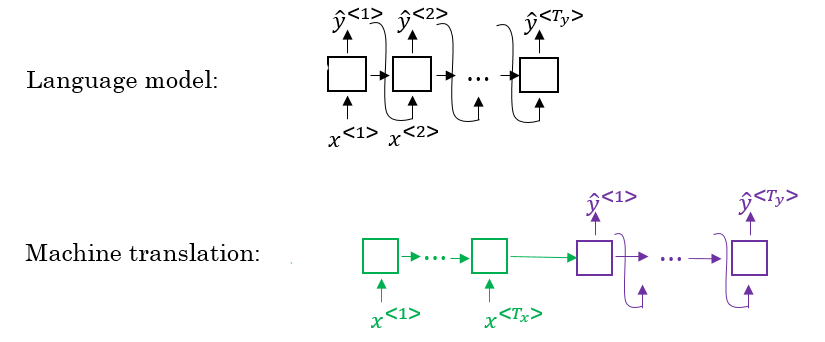
\includegraphics[width=5.0in]{55.png}\newline
\caption{Language model and machine translation with the same input and output lengths in our case

\label{fig:Lang_vs_Trans}}
\end{figure}
%%%%%%%%%%%%%%%%%%%%%%%%%
A conventional RNN is incapable of having long term dependencies that is to say if we have 
\subsection*{Machine Translation}
Although we will not be using Machine Translation in it's original form , but the idea behind using multi-layer LSTM to model the conditional probabilities can be understood by looking at a standard Ecoder-Decoder Model.
Let us denote the source sequence also called source phrase by $X=\left( x^{<1>},...,x^{<T_{x}>} \right)$
and a target sequence or target phrase by $Y=\left( y^{<1>},...,y^{<T_{y}>}\right)$. Each phrase is a sequence of $K$-dimensional one-hot vectors, such that only one element of the vector is $1$ and all the others are $0$. The index of the active ($1$) element indicates the word represented by the vector. For the simple case of 2 qubits, $T_{x}=T_{y}=16$ and $K=16$ since we are considering Pauli-4 measurements at each qubits and the dimensions in general will go as $K=2^{2N}$ where $N$ is the number of qubits and thus variables used in the above notation $T_{x}=T_{y}=N=16$. The reason to make the choice is because we want to learn all the $K=2^{2N}$ probabilities once we finish training.

\subsubsection*{Encoder}

Each term of the source phrase is embedded in a $16$-dimensional vector space:
$e(x^{<i>}) \in \mathbf{R}^{16}$.

In one of the many architectures used to model,
the hidden state of an encoder consists of $64$ hidden units, and each one of them at time $t$ is computed by

\begin{align}
    h_j^{\qt{t}} = z_j h_j^{\qt{t-1}} + (1 - z_j) \tilde{h}_j^{\qt{t}},
\end{align}
where  
\begin{align}
    \tilde{h}_j^{\qt{t}} =& \tanh\left( \left[ \textbf{W}_e(\textbf{x}^{<t>}) \right]_j + \left[\textbf{U} \left(\textbf{r}\odot \textbf{h}_{\qt{t-1}}\right) \right]_j \right)
    \\
    z_j =& \sigma\left( \left[\textbf{W}_z e(\textbf{x}^{<t>}) \right]_j + \left[\textbf{U}_{z} \textbf{h}_{\qt{t-1}}\right]_j \right)
    \\
    \label{eq:r}
    r_j =& \sigma\left( \left[ \textbf{W}_r e(\textbf{x}^{<t>}) \right]_j + 
    \left[\textbf{U}_{r} \textbf{h}_{\qt{t-1}}\right]_j \right)
\end{align}
$\sigma$ and $\odot$ are a logistic sigmoid function and an element-wise
multiplication (Note: $\vh_{<t-1>}$ is the whole set of the hidden units for the previous time step), respectively and $j$ is the $j^{th}$ hidden unit.
 Starting from the bottom \ref{eq:r}, the
\textit{reset} gate $r_j$ is computed by using $\sigma$ which is the logistic sigmoid function, and $\left[ . \right]_j$ denotes
the $j$-th element of a vector. $\vx$ and $\vh_{<t-1>}$ are the input and the
previous hidden state, respectively. $\mW_r$ and $\mU_r$ are weight matrices
which are learned.

Likewise, the \textit{update} gate $z_j$ is computed by
\begin{align*}
    \label{eq:update}
    z_j =& \sigma\left( \left[\textbf{W}_z e(\textbf{x}^{<t>}) \right]_j + \left[\textbf{U}_{z} \textbf{h}_{\qt{t-1}}\right]_j \right)
\end{align*}

The actual activation of the proposed unit $h_j$ is then computed by
\begin{align*}
    \label{eq:activation}
    h_j^{\qt{t}} = z_j h_j^{\qt{t-1}} + (1 - z_j) \tilde{h}_j^{\qt{t}},
\end{align*}
where
\begin{align*}
\label{eq:same_temp_hidden}
\tilde{h}_j^{\qt{t}} =& \tanh\left( \left[ \textbf{W}_e(\textbf{x}^{<t>}) \right]_j + \left[\textbf{U} \left(\textbf{r}\odot \textbf{h}_{\qt{t-1}}\right) \right]_j \right)
\end{align*}

In this formulation, when the reset gate is close to 0, the hidden state is
forced to ignore the previous hidden state and reset with the current input
only.

Once the hidden state at the $N$ step (the end of the source phrase) is computed, the representation of the source phrase
$\vc$ is
\begin{align*}
    \vc = \tanh \left( \mV \vh^{\qt{N}} \right).
\end{align*}

\subsubsection*{Decoder}

The decoder starts by initializing the hidden state with
\begin{align*}
    {\vh'}^{\qt{0}} = \tanh \left( \mV' \vc \right),
\end{align*}
where we will use $\cdot'$ to distinguish parameters of the
decoder from those of the encoder.

The hidden state at time $t$ of the decoder is computed by
\begin{align*}
    {h'}_j^{\qt{t}} = {z'}_j {h'}_j^{\qt{t-1}} +
    (1 - {z'}_j) \tilde{h'}_j^{\qt{t}},
\end{align*}
where
\begin{align*}
    \tilde{h'}_j^{\qt{t}} =& \tanh\left( 
    \left[ \mW' e(\vy_{t-1}) \right]_j + 
    {r'}_j \left[ \mU' {\vh'}_{\qt{t-1}} +
    \mC \vc 
    \right]
    \right),
    \\
    {z'}_j =& \sigma\left( \left[ {\mW'}_z e(\vy_{t-1}) \right]_j + 
    \left[{\mU'}_z {\vh'}_{\qt{t-1}}\right]_j +
    \left[\mC_z \vc \right]_j 
    \right),
    \\
    {r'}_j =& \sigma\left( \left[ {\mW'}_r e(\vy_{t-1}) \right]_j + 
    \left[{\mU'}_r {\vh'}_{\qt{t-1}}\right]_j +
    \left[ \mC_r \vc \right]_j
    \right)
\end{align*}
and $e(\vy_{0})$ is an all-zero vector. Similarly to the case of
the encoder, $e(\vy)$ is an embedding of a target word.

Unlike the encoder which simply encodes the source phrase, the
decoder is learned to generate a target phrase or give us the probability to go to a specific target phrase given we started with an input phrase. At each time $t$,
the decoder computes the probability of generating $j$-th word by $p(y_{t,j} = 1 \mid \vy_{t-1}, \dots, \vy_1, X)$ by applying a soft-max layer.
To draw a parallel between the parameters used in the actual implementations and the description, it is convenient to note that we have batch sizes of 10 which in the terminology of the machine translation will be like saying we have 10 different phrases of 1 word  say coming from 2 characters(number of qubits) and each of the characters(single qubit measurement) can come from a vocabulary of 4 (since we use Pauli-4 measurements). And once we flatten the two words the vocabulary is now $4\times4=16$. And each permutation of the two set of 4 letters has now been encoded into $16$ one hot vectors. Hence the shape of the output from a lstm layer would be (10,16,64) where 64 is a arbitrary choice of number of hidden nodes.
\begin{figure}[H]
    \centering
    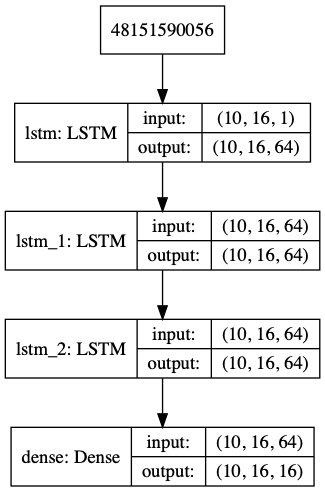
\includegraphics[width=3.0in]{model.png}
    \caption{The architecture of a model used consisting 3 LSTM layers which predicts the conditional probability for all the input cases}
    \label{fig:my_mdoel}
\end{figure}
The loss function used is KL-divergence which is defined by \begin{equation}
    \sum_{b_{1},b_{2}}P^{true}(b_{1}, b_{2} |a_{1}, a_{2})log(\frac{P^{true}(b_{1}, b_{2} |a_{1}, a_{2})}{P^{NN}(b_{1}, b_{2} |a_{1}, a_{2})})
\end{equation} where $P^{true}$ are the exact probabilities and $P^{NN}$ are the ones generated by the network. There are two kind of normalization that needs to be taken care of , one due to the fact that we are modelling the conditional probabilities here. For a given set of measurements all possible outcome probabilities will sum up-to 1. The other normalization that has been carefully chosen according to the batch size. To avoid aggressiveness of having Stochastic Gradient Descent (batch size=1), we use mini batch gradient where the descent is computed by the average of gradients over a batch of points in the neighbourhood of a training set. 
\pagebreak
\subsection*{Elementary Results}
\begin{figure}[H]
    \centering
    \subfloat[\textbf{a}]{{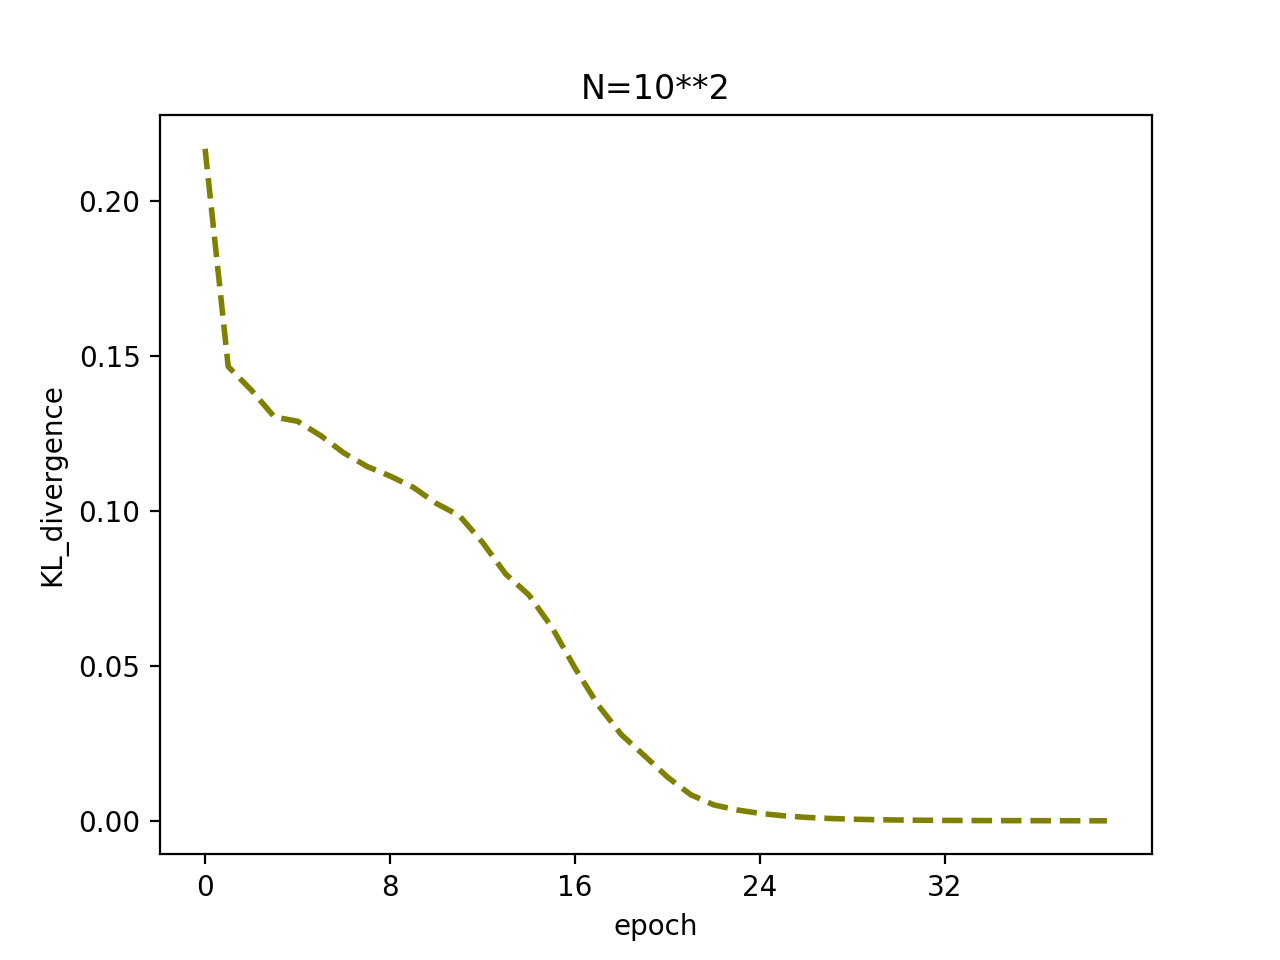
\includegraphics[width=7cm]{KL10_2.png} }}%
    \qquad
    \subfloat[\textbf{b}]{{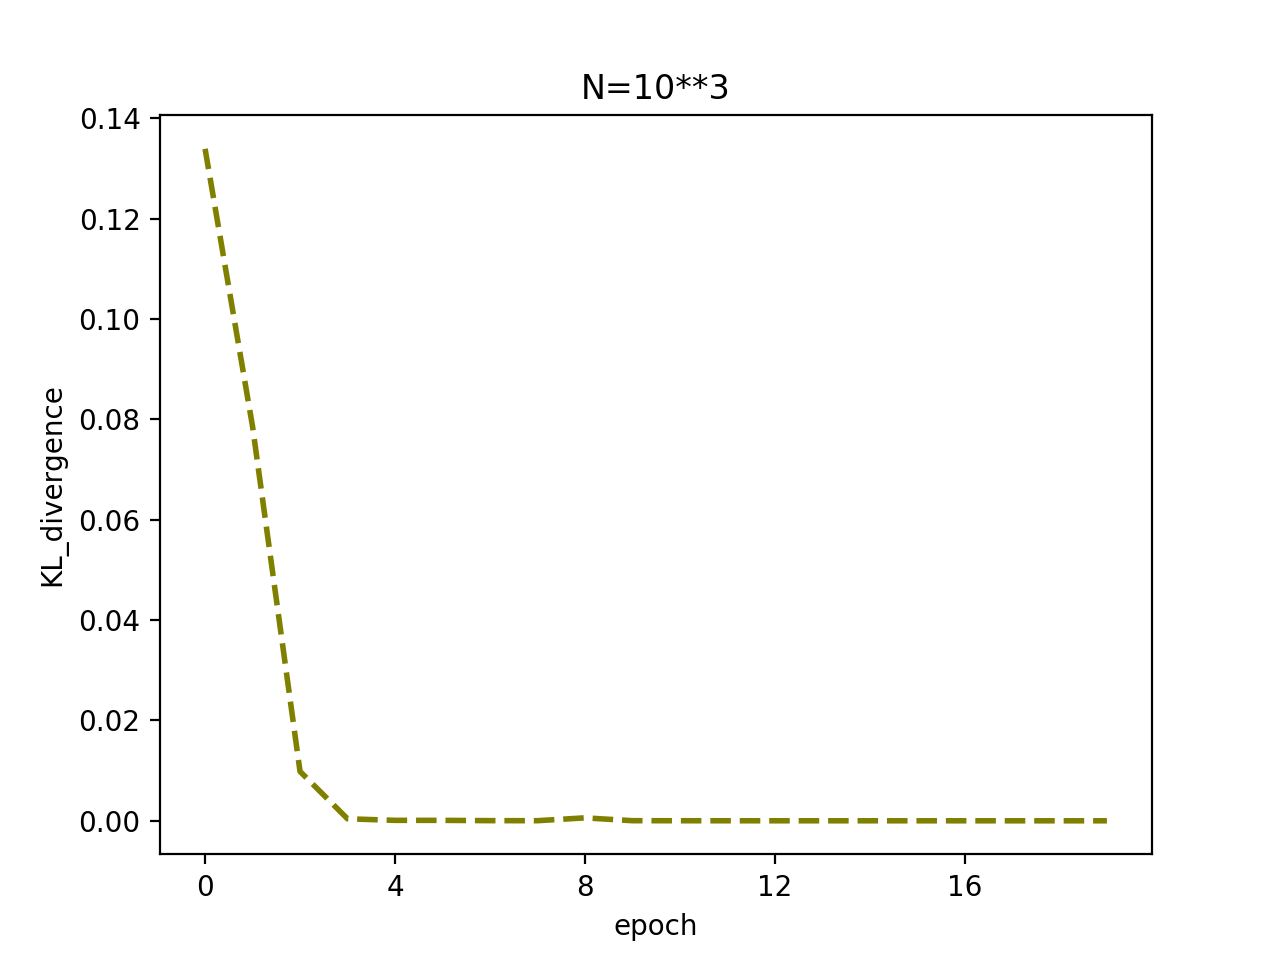
\includegraphics[width=7cm]{KL10_3.png} }}%
    \caption{Learning the conditional probabilities with two different number of samples}%
    \label{fig:example}%
\end{figure}
As discussed earlier the quantum fidelity defined between the  two  density  matrix  will  also  be  a  criteria  to  judge  the  training  that  we  perform  via  our neural network model. And for the case with 100 samples per given input states, we have a fidelity of \textbf{0.99x} after training the model with epoch greater than 30 and similarly with an increased number of samples($10^3$) we get \textbf{0.999x} after training the model for more than 10 epochs. These numbers are reported for a particular architecture with a fixed number of hidden nodes in each layer and a specific batch size.

\begin{thebibliography}{9}
\bibitem{11},  \textit{}.
\end{thebibliography}
\end{document}
